\documentclass[10pt,landscape]{article}
\usepackage{multicol}
\usepackage{graphicx}
\usepackage{calc}
\usepackage{ifthen}
\usepackage{color}
\usepackage[landscape]{geometry}

\ifthenelse{\lengthtest { \paperwidth = 11in}}
	{ \geometry{top=.05in,left=.2in,right=0in,bottom=.05in} }
	{\ifthenelse{ \lengthtest{ \paperwidth = 297mm}}
		{\geometry{top=1cm,left=1cm,right=1cm,bottom=1cm} }
		{\geometry{top=1cm,left=1cm,right=1cm,bottom=1cm} }
	}

% Turn off header and footer
\pagestyle{empty}
 

% Redefine section commands to use less space
\makeatletter
\renewcommand{\section}{\@startsection{section}{1}{0mm}%
                                {-1ex plus -.5ex minus -.2ex}%
                                {0.5ex plus .2ex}%x
                                {\normalfont\large\bfseries}}
\renewcommand{\subsection}{\@startsection{subsection}{2}{0mm}%
                                {-1explus -.5ex minus -.2ex}%
                                {0.5ex plus .2ex}%
                                {\normalfont\normalsize\bfseries}}
\renewcommand{\subsubsection}{\@startsection{subsubsection}{3}{0mm}%
                                {-1ex plus -.5ex minus -.2ex}%
                                {1ex plus .2ex}%
                                {\normalfont\small\bfseries}}
\makeatother

% Define BibTeX command
\def\BibTeX{{\rm B\kern-.05em{\sc i\kern-.025em b}\kern-.08em
    T\kern-.1667em\lower.7ex\hbox{E}\kern-.125emX}}

% Don't print section numbers
\setcounter{secnumdepth}{0}


\setlength{\parindent}{0pt}
\setlength{\parskip}{0pt plus 0.5ex}


\newlength{\MyLen}
\settowidth{\MyLen}{\texttt{letterpaper}/\texttt{a4paper} \ }
% -----------------------------------------------------------------------

\begin{document}

\raggedright
\footnotesize
\begin{multicols}{3}
\vspace{-5mm}
\begin{center}
\includegraphics[width=198.5px]{header.png}\end{center}
\setlength{\premulticols}{1pt}
\setlength{\postmulticols}{1pt}
\setlength{\multicolsep}{1pt}
\setlength{\columnsep}{2pt}

\section{Standard navigation keys}

Many readline keyboard shortcuts work in \textit{emergent} and can
greatly enhance productivity. The rest of this section shows how to
interpret the \textit{Standard} rows for all of the following sections. On OSX
you can swap the Cmd and Ctrl (\verb!^!) keys and Cmd+v is paste while \verb!^!v is
Page Down.\\~\\
\begin{tabular}{@{}ll@{}}
\verb!Tab/Shift+Tab! & Forward/Backwards through elements/interface\\
\verb!Page Up/Down!    & Move cursor to the top/bottom or first/last element\\
\verb!^Space!    & Enable select as you navigate mode.\\
\verb!^f!    & Move cursor forwards or expand node.\\
\verb!^b!    & Move cursor backwards or collapse node.\\
\verb!^n!    & Move cursor down one line. (Use with \verb!^!Space) \\
\verb!^p!    & Move cursor up one line. (Use with \verb!^!Space)\\
\verb!^a!    & Move cursor to first character of line\\
\verb!^e!    & Move cursor to last character of line\\
\verb!^d!  & Delete item in focus or all selected items.\\
\verb!^g!  & Deselect text or tree selection.\\
\verb!^x, ^w! & Cut.\\
\verb!^c, Alt+w! & Copy.\\
\verb!^v, ^y! & Paste.
\end{tabular}

\section{css console and text fields}

\begin{tabular}{@{}ll@{}}
\verb!Standard!  & \verb!^!f/b/n/p/a/e/d/x/w/c/v/y. \\
\verb!^k! & Put text from cursor to end of line on clipboard.\\
\verb!^y! & Paste text from clipboard.\\
\verb!^l! & Clear buffer.\\
\verb!^!$\rightarrow$ & Move cursor one word forward. \\
\verb!^!$\leftarrow$ & Move cursor one word backwards. \\
\verb!^Shift!$\rightarrow$ & Highlight one word forward. \\
\verb!^Shift!$\leftarrow$ & Highlight one word backwards.\\
\verb!On Mac Opt+! & Use option instead of control.
\end{tabular}

\section{Global project}

\begin{tabular}{@{}ll@{}}
\verb!Standard!    & Tab \\
\verb!^s!    & Save project (Mac Cmd+s). \\
\verb!^!$\leftarrow$ & Backwards in navigation history \\
\verb!^!$\rightarrow$ & Forwards in navigation history \\
\verb!F5!  & Refresh GUI. \\
\verb!^j,Alt+j! & Move global focus left \\
\verb!^l,Alt+l! & Move global focus right
\end{tabular}

\section{Window frames}

\begin{tabular}{@{}ll@{}}
\verb!^1!    & Tree browser only \\
\verb!^2!    & Panel frame only \\
\verb!^3!    & Tree \& panel frame \\
\verb!^4!    & 3D frame only \\
\verb!^5!    & Tree \& 3D frame \\
\verb!^6!    & Panels \& 3D frame \\
\verb!^7!    & All frames \\
\end{tabular}

\section{Control over Program run state}

\begin{tabular}{@{}ll@{}}
\verb!Init,Run,Step,Stop,Abort!    & F8,F9,F10,F11,F12
\end{tabular}

\section{Help Browser}

\begin{tabular}{@{}ll@{}}
\verb!Standard!  & Tab,Page,\verb!^!f/b/n/p/a/e/x/w/c/y/v. \\
\verb!F1!  & Help Browser. \\
\verb!^s!  & Toggle Search/Find focus.
\\
\\
\end{tabular}

\section{Project tree and program tree}

\settowidth{\MyLen}{\texttt{multicol}}
\begin{tabular}{@{}ll@{}}
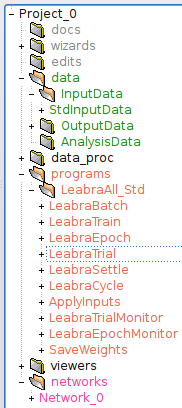
\includegraphics[width=91px]{treebrowser.png}   & 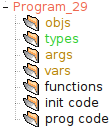
\includegraphics[width=150px]{programcode.png}
\end{tabular}
\begin{tabular}{@{}ll@{}}
\verb!Standard!    & Page,\verb!^!Space/f/b/n/p/d/g/x/w/c/v/y. \\
\verb!Any 1-3 chars!    & Find as you type.\\
\verb!^i!    & New item below cursor. \\
\verb!Alt+f!  & Find from selected node. \\
\verb!^m!  & Duplicate element(s).
\end{tabular}

\subsection{New items in the project tree}

Find as you type works in project trees and is useful for creating new
objects. For example, \textit{da} followed by Enter (no chooser) or
\verb!^i! (chooser) will create a new datatable. You can then press
\verb!^!$\leftarrow$ to navigate back to where you were. Examples:

\begin{tabular}{@{}ll@{}}
\verb!da Enter!    & New DataTable \\
\verb!pr Enter!    & New Program \\
\end{tabular}
\\

\subsection{New items in the program tree}

Find as you type also works in program trees. For example, to create a
new variable type \textit{var Enter}, or to create a new object of a
specific type, type \textit{obj} \verb!^i!. Examples:

\begin{tabular}{@{}ll@{}}
\verb!obj ^i Type!    & New obj \\
\verb!var ^i!    & New var \\
\verb!fun ^i!    & New fun \\
\end{tabular}
\\

\subsection{Text fields}


\includegraphics[width=205px]{path.png} \\
\begin{tabular}{@{}ll@{}}
\verb!^l!    & Text completion lookup.  \\
\verb!^u!    & Highlight all.
\end{tabular}
\\~\\
\columnbreak

\section{Edit panels}
See the ``Text fields'' section for shortcuts that work on the text
fields of edit panels.
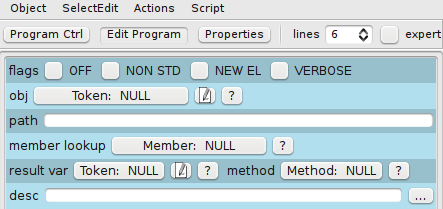
\includegraphics[width=221.5px]{middlepanel.png}
\\ \settowidth{\MyLen}{\texttt{multicol} }
\begin{tabular}{@{}ll@{}} \\
\verb!Standard!    & Tab  \\
$\uparrow\downarrow$    & (numeric field) Increase/decrease value. \\
$\uparrow\downarrow$    & (dropdown) Move up/down. \\
\verb!First Character!    & (dropdown) Selects item. \\
\verb!ESC!    & Revert text field changes. \\
\verb!^Enter!    & Apply changes. \\
\verb!Space!    & Open token chooser and Check/uncheck flag.\\
\verb!^l!    & (expression fields) Lookup information.
\end{tabular}

\section{DataTables and matrices}
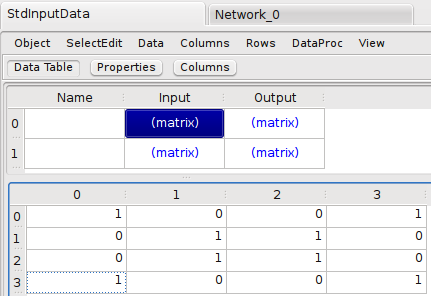
\includegraphics[width=215.5px]{datatable.png}
\begin{tabular}{@{}ll@{}}
\verb!Standard!  & Page,\verb!^!f/b/n/p/a/e/c/v/d/g/y.\\
\verb!^t!    & Switch between table and matrix focus. \\
\verb!^i!    & Insert new row before selected row. \\
\verb!^m!    & Duplicate row. \\
\verb!^Space!    & Start editing cell.
\end{tabular}

\section{Choosers}
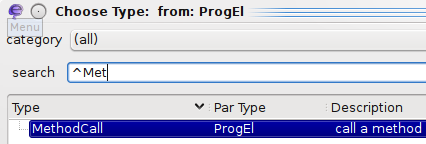
\includegraphics[width=213px]{progel.png} \\
\begin{tabular}{@{}ll@{}}
\verb!Standard!  & Tab,\verb!^!f/b/n/p/a/e/d/x/w/c/v/y.
\end{tabular}

\section{3D View}
\begin{tabular}{@{}ll@{}}
\verb!Arrow keys!    & Rotate\\
\verb!Shift + Arrow keys!    & Pan\\
\verb!-!    & Zoom-Out\\
\verb!+ or =! & Zoom-In.
\end{tabular}

\end{multicols}

\end{document}
